\chapter{UI Prototypes}\label{ch:ui_prototypes}

\section{Prototype 1}

\begin{figure}[h]
  \centering
  \begin{subfigure}[b]{0.3\textwidth} % Reduced width for 3 images per row
    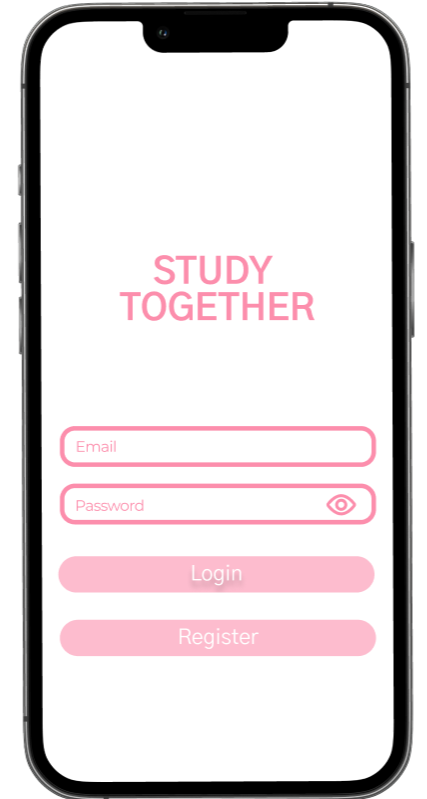
\includegraphics[width=\textwidth]{Figures/landing.png}
    \caption{Landing Page}
    \label{fig:landing}
  \end{subfigure}
  \hfill
  \begin{subfigure}[b]{0.3\textwidth}
    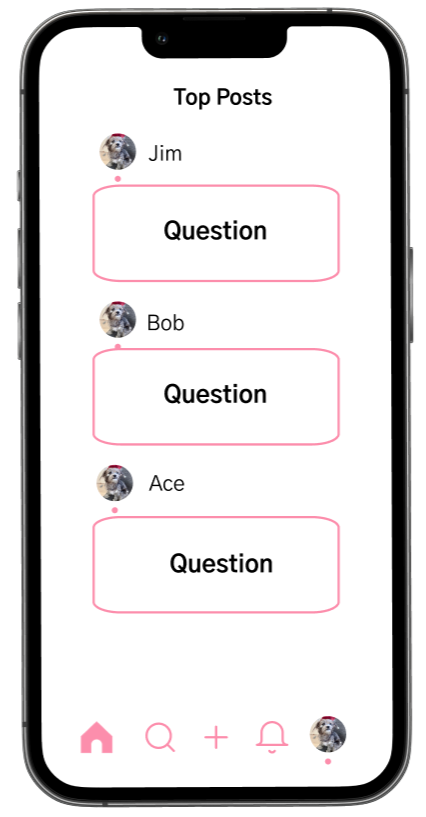
\includegraphics[width=\textwidth]{Figures/home.png}
    \caption{Home Page}
    \label{fig:home}
  \end{subfigure}
  \hfill
  \begin{subfigure}[b]{0.3\textwidth}
    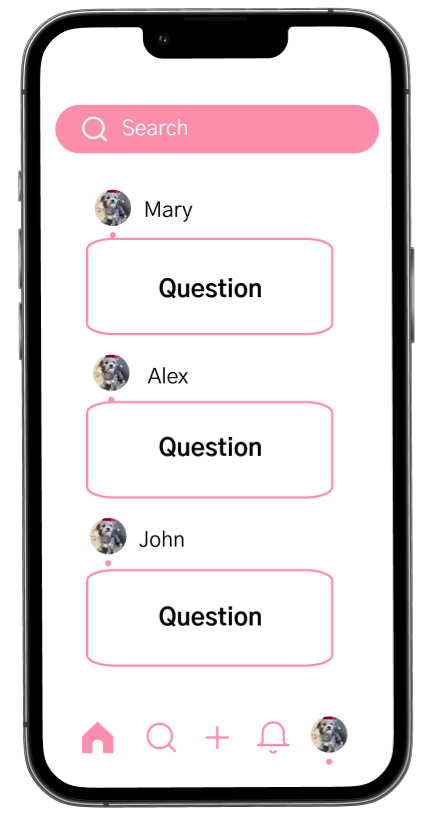
\includegraphics[width=\textwidth]{Figures/search.png}
    \caption{Search Page}
    \label{fig:search}
  \end{subfigure}
  \label{fig:prototype1_screens_1}
  \caption{Key screens of Prototype 1, showcasing various UI elements and interactions for the mobile app.}
\end{figure}

\begin{figure}[h]
  \begin{subfigure}[b]{0.3\textwidth}
    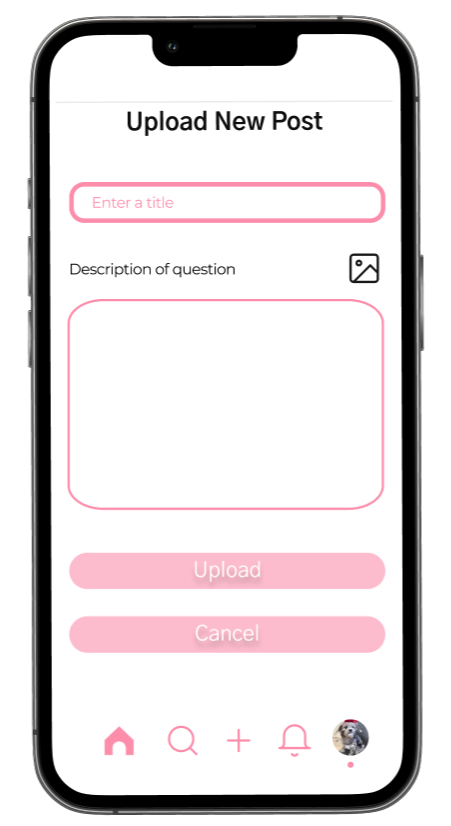
\includegraphics[width=\textwidth]{Figures/upload.png}
    \caption{Upload Page}
    \label{fig:upload}
  \end{subfigure}
  \hfill
  \begin{subfigure}[b]{0.3\textwidth}
    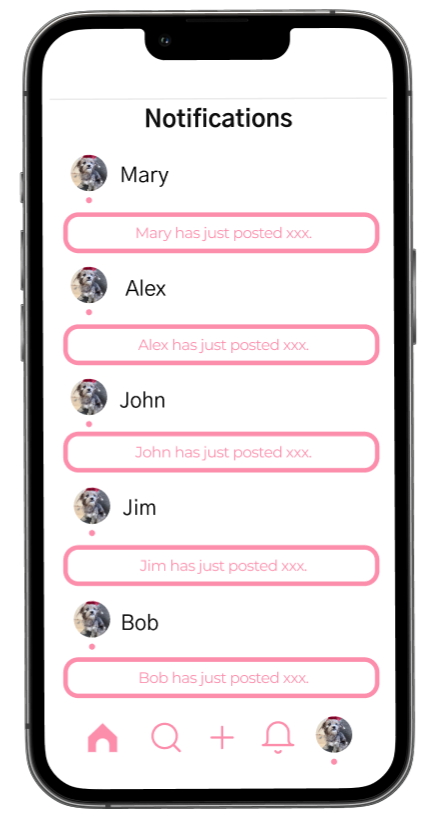
\includegraphics[width=\textwidth]{Figures/notification.png}
    \caption{Notification Page}
    \label{fig:notification}
  \end{subfigure}
  \hfill
  \begin{subfigure}[b]{0.3\textwidth}
    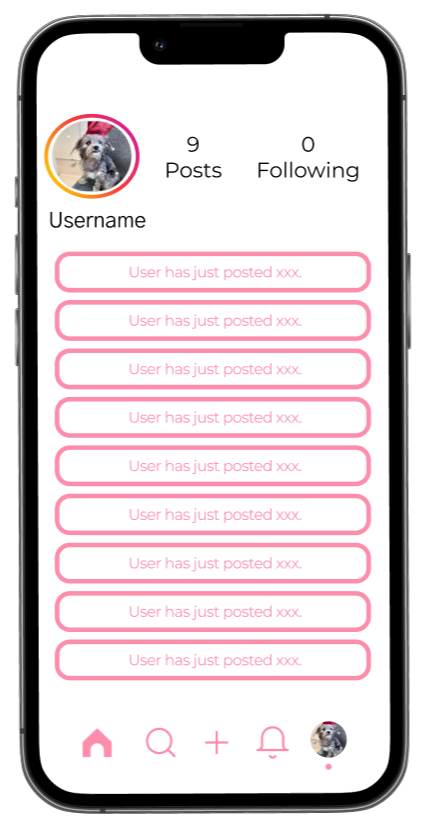
\includegraphics[width=\textwidth]{Figures/profile.png}
    \caption{Profile Page}
    \label{fig:profile}
  \end{subfigure}
  \caption{Key screens of Prototype 1, showcasing various UI elements and interactions for the mobile app.}
  \label{fig:prototype1_screens_2}
\end{figure}
